\documentclass[11pt]{article}

% ==== PACKAGES ==== %
% \usepackage{fullpage}
\usepackage{amsmath,amssymb,amsthm}
\usepackage{epic}
\usepackage{eepic}
\usepackage{hyperref}
\usepackage{listings}
\usepackage{float}
\usepackage{graphicx}
\usepackage{fancyhdr}
\usepackage{color}
\usepackage{bbm}
\usepackage[letterpaper, margin=1in]{geometry}

% ==== MARGINS ==== %
% \pagestyle{empty}
% \setlength{\oddsidemargin}{0in}
% \setlength{\textwidth}{6.8in}
% \setlength{\textheight}{9.5in}

\pagestyle{fancy}
\fancyhf{}
\rhead{ASEN 5044}
\lhead{Homework 1}
\rfoot{Page \thepage}


\newtheorem*{solution*}{Solution}
\newtheorem{lemma}{Lemma}[section]
\newtheorem{theorem}[lemma]{Theorem}
\newtheorem{claim}[lemma]{Claim}
\newtheorem{definition}[lemma]{Definition}
\newtheorem{corollary}[lemma]{Corollary}
\lstset{moredelim=[is][\bfseries]{[*}{*]}}

% ==== DOCUMENT PROPER ==== %
\begin{document}

\thispagestyle{empty}

% --- Header Box --- %
\newlength{\boxlength}\setlength{\boxlength}{\textwidth}
\addtolength{\boxlength}{-4mm}

\begin{center}\framebox{\parbox{\boxlength}{\bf
      Statistical Estimation \hfill Homework 1\\
      ASEN 5044 Fall 2018 \hfill Due Date: Sep 6, 2018\\
      Name: Andrew Kramer \hfill PhD Student
}}
\end{center}




\section*{Exercise 1}

Compute determinants for the following matrices by hand and state whether each one is invertible

\subsection*{Problem (a)}

\subparagraph*{}

\begin{align*}
	|A| &= 1 \begin{vmatrix} 5 & 4 \\ 9 & 7 \end{vmatrix} - 2 \begin{vmatrix} 6 & 4 \\ 8 & 7 \end{vmatrix} + 3 \begin{vmatrix} 6 & 5 \\ 8 & 9 \end{vmatrix} \\
	&= 1(-1) - 2(10) + 3(14) \\
	&= 21
\end{align*}

Because $|A|$ is nonzero $A$ is invertible.

\subsection*{Problem (b)}

\subparagraph*{}

\begin{align*}
	|A| &= 11 \begin{vmatrix} 57 & 0 & 10 \\ 91 & 1 & 71 \\ 23 & 0 & 71 \end{vmatrix} - 26 \begin{vmatrix} 64 & 0 & 10 \\ 83 & 1 & 71 \\ 54 & 0 & 71 \end{vmatrix} \\
	&= 11(57(71) + 10(-23)) - 26(64(71)+10(-54)) \\
	&= 41978 - 109642 \\
	&= -67655
\end{align*}

Because $|A|$ is nonzero $A$ is invertible.

\subsection*{Problem (c)}

\subparagraph*{}

Because $A_1 = -2A_3$ (where $A_i$ refers to the $i^\text{th}$ column of A), the columns of A are not linearly independent. This means $A$ is not invertible and $|A| = 0$.

\subsection*{Problem (d)}

\subparagraph*{}

Because the determinant of an upper triangular matrix is simply the product of its diagonal elements:
\begin{align*}
	|A| &= 1 \times 8 \times 55 \times 233 \times 610 \\
	&= 62537200
\end{align*}

Because $|A|$ is nonzero $A$ is invertible.

\section*{Exercise 2}
Prove each of the following statements:
\subsection*{Problem (a)}
If $a$ and $b$ are non-zero $n\times 1$ vectors, then the matrix $ab^T$ has rank $1$.
\subparagraph*{}
Column $i$ of the outer product of $a$ and $b$ is simply the vector $a$ multiplied by the scalar $b_i$. This means that every column of $ab^T$ is a scalar multiple of $a$, so none of the columns of $ab^T$ are linearly independent. Thus, the rank of $ab^T$ is always one if both $a$ and $b$ are nonzero.
\subsection*{Problem (b)}
$\text{tr}(AB) = \text{tr}(BA)$ if $A$ is an $m\times n$ matrix and $B$ is $n\times m$.
\subparagraph*{}
The trace of $AB$ can be expressed as 
\begin{align*}
	\text{tr}(AB) &= \sum_{i=1}^n(AB)_{ii} \\
	&= \sum_{i=1}^n \sum_{j=1}^n a_{ij}b_{ji}
\end{align*} 
Similarly, the trace of $BA$ is
\begin{align*}
	\text{tr}(BA) &= \sum_{j=1}^n(BA)_{jj} \\
	&= \sum_{j=1}^n \sum_{i=1}^n b_{ji}a_{ij}
\end{align*}
Because $\sum_{i=1}^n \sum_{j=1}^n a_{ij}b_{ji}$ is equal to $\sum_{j=1}^n \sum_{i=1}^n b_{ji}a_{ij}$ we can conclude that $\text{tr}(AB) = \text{tr}(BA)$.
\subsection*{Problem (c)}
If $A$ is invertible then $|A^{-1}| = \frac{1}{|A|}$.
\subparagraph*{}
If we start with $|AB| = |BA| = |A|\ |B|$ and replace $B$ with $A^{-1}$ we find that 
\begin{align*}
	|A|\ |A^{-1}| &= |AA^{-1}| \\
	&= |I| \\
	&= 1
\end{align*}
Because $|A|\ |A^{-1}| = 1$ it must be true that $|A^{-1}| = \frac{1}{|A|}$. 

\section*{Exercise 3}
Consider the equations of motion for the coupled $2$ mass $3$ spring system like the one discussed in lecture. Find a set of $A,B,C,D$ matrices for the state vector definition,
\begin{equation*}
	x = [q_1-q_2,\ \dot{q}_1-\dot{q}_2,\ q_1+q_2,\ \dot{q}_1+\dot{q}_2]^T 
\end{equation*}
and for observations $y=[q_1,\ q_2]^T$ and inputs $u=[u_1,\ u_2]^T$.

\subparagraph{}
The following solution makes the assumption, as was done in lecture, that $m_1 = m_2 = 1\text{kg}$ and $k_1 = k_2 = k_3 = 1\text{N/m}$.

\begin{align*}
	\ddot{q}_1 &= -q_1 - q_1 + q_2 - u_1 \\
	&= -2q_1 + q_2 - u_1 \\
	\ddot{q}_2 &= -q_2 + q_1 - q_2 + u_1 + u_2 \\
	&= -2q_2 + q_1 + u_1 + u_2 \\
	\ddot{q}_1-\ddot{q}_2 &= (-2q_1+q_2-u_1) - (q_1-2q_2+u_1+u_2) \\
	&= -3q_1 + 3q_2 - 2u_1 - u_2 \\
	&= -3(q_1 - q_2) -2u_1 - u_2 \\
	\ddot{q}_1+\ddot{q}_2 &= (-2q_1+q_2-u_1) + (q_1-2q_2+u_1+u_2) \\
	&= -q_1 - q_2 + u_2 \\
	&= -(q_1 + q_2) + u_2 
\end{align*}

From these results we can construct our $A,B,C$, and $D$ matrices as follows:

\begin{equation*}
	A=\begin{bmatrix} 0&1&0&0\\-3&0&0&0 \\ 0&0&0&1 \\ 0&0&-1&0 \end{bmatrix}\quad B=\begin{bmatrix} 0&0 \\ -2&-1 \\ 0&0 \\ 0&1 \end{bmatrix}\quad C=\begin{bmatrix} \frac{1}{2}&0&\frac{1}{2}&0 \\ -\frac{1}{2}&0&-\frac{1}{2}&0 \end{bmatrix}\quad D=\begin{bmatrix} 0&0 \\ 0&0 \end{bmatrix}
\end{equation*}

\section*{Exercise 4}
The linearized equations of motion for an orbiting satellite spinning with nominal angular rate $p_o$ about the x axis are
\begin{align*}
	\Delta\dot{p} &= \frac{M_x}{I_x} \\
	\Delta\dot{q} &= \frac{p_0(I_x-I_z)\Delta r + M_y}{I_y} \\
	\Delta\dot{r} &= \frac{p_0(I_y-I_x)\Delta q + M_z}{I_z}
\end{align*}
where $I_x,I_y,$ and $I_z$ are the moments of inertia about the roll, pitch, and yaw axes; $M_x,M_y,$ and $M_z$ are the corresponding input torques; and $\Delta p,\Delta q,$ and $\Delta r$ are perturbations in rolling, pitching, and yawing rates from the linearization point.

\subsection*{Problem (a)}
Using the state vector $x = [\Delta p, \Delta q, \Delta r]^T$, input vector $u = [M_x,M_y,M_z]^T$, and output vector $y=x$, put this system into state space form.

\subparagraph{}
The state space form of the given system is as follows:
\begin{equation*}
	A = \begin{bmatrix} 
		0 & 0 & 0 \\
		0 & 0 & \frac{p_o(I_x-I_z)}{I_y} \\
		0 & \frac{p_o(I_y-I_x)}{I_z} & 0
	\end{bmatrix} \quad 
	B = \begin{bmatrix}
		\frac{1}{I_x} & 0 & 0 \\
		0 & \frac{1}{I_y} & 0 \\
		0 & 0 & \frac{1}{I_z}
	\end{bmatrix} \quad
	C = \mathbb{I}_3 \quad 
	D = 0_3
\end{equation*}

\subsection*{Problem (b)}
Use Matlab's \texttt{expm} function to compute the state transition matrix for this system assuming that $I_y=750\text{kg m}^3$, $I_z=1000\text{kg m}^3$, $I_x=500 \text{kg m}^3$, $p_0 = 20 \text{rad/s}$, and $\Delta t=0.1\text{s}$.

\subparagraph*{}
\begin{equation*}
	e^{A\Delta t} = \begin{bmatrix}
					1 & 0 & 0 \\
					0 & 0.685 & -1.19 \\
					0 & 0.446 & 0.685
					\end{bmatrix}
\end{equation*}

\subsection*{Problem (c)}
Use the state transition matrix to compute and plot the state time history for 5s, assuming zero inputs and assuming initial states $\Delta q(0) = 0.1\text{rad/s}$, and $\Delta p(0) = \Delta r = 0$. What can you say about the behavior of this system in terms of stability?

\subparagraph*{}
As figure \ref{fig:prob4} above shows, the system is asymptotically stable in $\Delta p$ and marginally stable in $\Delta q$ and $\Delta r$. $\Delta q$ is bounded between $-0.1$ and $0.1$ and $\Delta r$ is bounded between $-0.06$ and $0.06$.

\begin{figure}
	\centerline{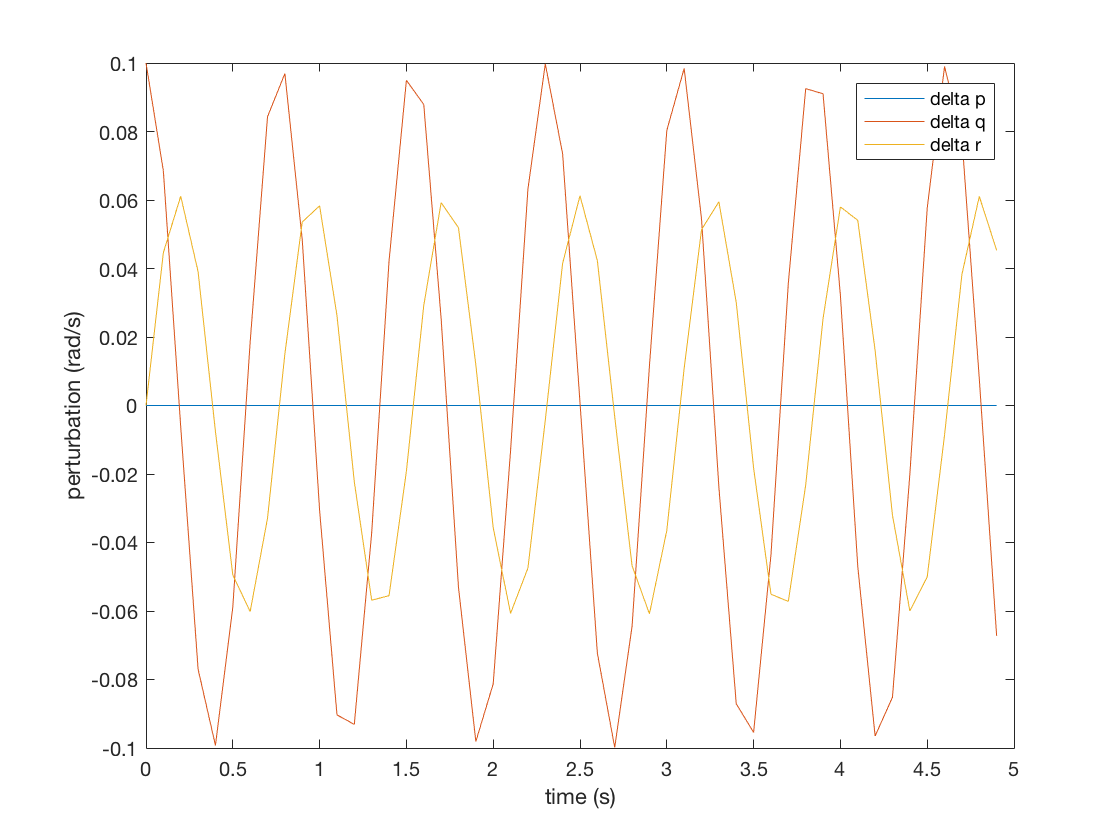
\includegraphics[width=0.67\linewidth]{prob_4_fig.png}}
	\caption{State variables plotted over time (exercise 4)}
	\label{fig:prob4}
\end{figure}

\section*{Exercise 5}
\subsection*{Problem (a)}
Consider the matrix 
\begin{equation*}
	A=\begin{bmatrix} a & b \\ b & c \end{bmatrix}
\end{equation*}
Recall that the eigenvalues af $A$ are found by finding the roots of the polynomial $P(\lambda)=|\lambda I-A|$. Show that $P(A)=0$.
\subparagraph*{}
The characteristic polynomial $p(\lambda)$ of $A$ is $|\lambda I - A| = \lambda^2 + \lambda(-a-c) + ac - b^2$. So 
\begin{align*}
	p(A) &= A^2 + A(-a-c) + I(ac-b^2) \\
	&= \begin{bmatrix} a^2+b^2 & ab+bc \\ ab+bc & b^2+c^2 \end{bmatrix}+
	\begin{bmatrix} -a^2-ac & -ab-bc \\ -ab-bc & -ac-c^2 \end{bmatrix}+
	\begin{bmatrix} ac-b^2 & 0 \\ 0 & ac-b^2 \end{bmatrix} \\
	&= \begin{bmatrix} 0 & 0 \\ 0 & 0 \end{bmatrix}
\end{align*}

\subsection*{Problem (b)}
Consider the matrix
\begin{equation*}
	A=\begin{bmatrix} a & b \\ b & c \end{bmatrix}
\end{equation*}
where $a,b,$ and $c$ are real and $a$ and $c$ are nonnegative. Compute the solutions of the characteristic polynomial of $A$ to prove that the eigenvalues of $A$ are real. Also, for what values of $b$ is $A$ positive semidefinite?
\subparagraph*{}
The characteristic polynomial $p(\lambda)$ of $A$ is $|\lambda I - A| = \lambda^2 + \lambda(-a-c) + ac - b^2$. The roots of this polynomial are given by the quadratic formula:
\begin{align*}
	\lambda &= \frac{-(-a-c)\pm\sqrt{(-a-c)^2-4(ac-b^2)}}{2} \\
	&= \frac{(a+c)\pm\sqrt{(a-c)^2+4b^2}}{2}
\end{align*}
Notice that the polynomial's discriminant (the expression under the radical) is the sum of the squares of real numbers. This means the discriminant is always positive and hence the roots of the characteristic polynomial (which are also the eigenvalues of $A$) are always real.\\
$A$ is positive semidefinite if $z^TAz \geq 0$ for every $z \in \mathbb{R}^2$. 
\begin{equation*}
	z^TAz=z_1^2a + 2z_1z_2b + z_2^2c
\end{equation*}
Since $a$ and $c$ are nonnegative $z_1^2a \geq 0$ and $z_2^2c \geq 0$. This means for $A$ to be positive semidefinite we only need to guarantee that $z_1z_2b \geq 0$. This is true if $z_1$ and $z_2$ have the same sign and $b \geq 0$ or if $z_1$ and $z_2$ have opposite signs and $b\leq0$. So the only value of $b$ that guarantees that $z^TAz\geq0$ for all $z\in\mathbb{R}^2$ is $0$. \\
There are other values of b that result in a positive semidefinite $A$ matrix. $A$ is positive semidefinite if its eigenvalues are nonnegative. We can find the values of $b$ which result in nonnegative roots to the characteristic polynomial:
\begin{equation*}
	(a+c)\pm\sqrt{(a-c)^2+4b^2} \geq 0
\end{equation*}
We first find the values of $b$ for which the above inequality is true when the square root is subtracted:
\begin{align*}
	-\sqrt{(a-c)^2+4b^2} &\geq -(a+c) \\
	\sqrt{(a-c)^2+4b^2} &\leq (a+c) \\
	(a-c)^2+4b^2 &\leq (a+c)^2 \\
	4b^2 &\leq (a+c)^2 - (a-c)^2 \\
	4b^2 &\leq a^2+2ac+c^2-a^2+2ac-c^2 \\
	4b^2 &\leq 4ac \\
	b &\leq \sqrt{ac}
\end{align*}
Then we find the values of $b$ for which the inequality holds when the square root is added:
\begin{align*}
	\sqrt{(a-c)^2+4b^2} &\geq -(a+c) \\
	(a-c)^2+4b^2 &\geq (-a-c)^2 \\
	4b^2 &\geq (-a-c)^2 - (a-c)^2 \\
	4b^2 &\geq a^2+2ac+c^2-a^2+2ac-c^2 \\
	b &\geq \sqrt{ac}
\end{align*}
So $A$ is positive semidefinite when $b\geq\sqrt{ac}$, $b\leq\sqrt{ac}$, and $b=0$.

\section*{Exercise AQ1}
Explain why matrix element $(4,4)$ in problem 1c belongs in the last column.
\subparagraph*{}
The number $42$ is the answer to life, the universe, and everything. Because a single, numerical answer to life, the universe, and everything is an irrational concept it belongs in the column composed of irrational numbers.

\section*{Exercise AQ2}
Using the infinite series definition of the matrix exponential, find the analytical expression for the state transition matrix of the spinning satellite system in problem $4$, assuming a generic value for $\Delta t$ and using the values for $I_x$, $I_y$, $I_z$, and $p_0$ given in that problem. Your answer should be a function of $\Delta t$. 

\subparagraph{}
When we expand the first few terms of the infinite series for $e^{A\Delta t}$ we get
\begin{align*}
	\sum_{i=0}^4 \frac{(A\Delta t)^i}{i!} &= I + A\Delta t + \frac{(A\Delta t)^2}{2!} + \frac{A\Delta t)^3}{3!} + \frac{(A\Delta t)^4}{4!} \\
	&= \begin{bmatrix} 1 & 0 & 0 \\
					   0 & 1 & 0 \\
					   0 & 0 & 1 \end{bmatrix} + 
	   \begin{bmatrix} 0 & 0 & 0 \\
	   				   0 & 0 & -13.333\Delta t \\
	   				   0 & 5\Delta t & 0 \end{bmatrix} 
	   + \frac{1}{2!} 
	   \begin{bmatrix} 0 & 0 & 0 \\
	   				   0 & 66.667\Delta t^2 & 0 \\
	   				   0 & 0 & 66.667\Delta t^2 \end{bmatrix} \\
	   &\qquad + \frac{1}{3!}
	   \begin{bmatrix} 0 & 0 & 0 \\
	   				   0 & 0 & 888.9\Delta t^3 \\
	   				   0 & -333.3\Delta t^3 & 0 \end{bmatrix}
	   + \frac{1}{4!}
	   \begin{bmatrix} 0 & 0 & 0 \\
	   				   0 & 4444\Delta t^4 & 0 \\
	   				   0 & 0 & 4444\Delta t^4 \end{bmatrix}
\end{align*}
We can see the nonzero terms in the sum above, which I'll refer to as $\phi$, are
\begin{align*}
	\phi_{1,1} &= 1 \\
	\phi_{2,2} = \phi_{3,3} &= 1-\frac{66.666}{2!}\Delta t^2 + \frac{4444}{4!}\Delta t^4 \\
	&= 1 - \frac{8.17^2}{2!}\Delta t^2 + \frac{8.17^4}{4!}\Delta t^4 \\
	\phi_{2,3} &= -13.333\Delta t + \frac{888.9}{3!}\Delta t^3 \\
	&= -1.63 \Big[8.17\Delta t + \frac{8.17^3}{3!}\Delta t^3 \Big] \\
	\phi_{3,2} &= 5\Delta t - \frac{333.3}{3!}\Delta t^3 \\
	&= 0.612 \Big[8.17\Delta t + \frac{8.17^3}{3!}\Delta t^3 \Big]
\end{align*}
Noting that the Taylor series expansion of $a\cos(bx) = a[1-\frac{(bx)^2}{2!}+\frac{(bx)^4}{4!} - \dots]$ and the expansion of $a\sin(bx) = a[bx-\frac{(bx)^3}{3!} + ...]$ we can deduce that $e^{A\Delta t}$ is equal to
\begin{equation*}
	e^{A\Delta t} = \begin{bmatrix} 1 & 0 & 0 \\
		0 & \cos(8.17\Delta t) & -1.63\sin(8.17\Delta t) \\
		0 & 0.612\sin(8.17\Delta t) & \cos(8.17\Delta t)
		\end{bmatrix}
\end{equation*}

\end{document}
